% !TEX TS-program = pdflatex
\documentclass[10pt,twocolumn]{article} 

% required packages for Oxy Comps style
\usepackage{oxycomps} % the main oxycomps style file
\usepackage{times} % use Times as the default font
\usepackage[style=numeric,sorting=nyt]{biblatex} % format the bibliography nicely 

\usepackage{amsfonts} % provides many math symbols/fonts
\usepackage{listings} % provides the lstlisting environment
\usepackage{amssymb} % provides many math symbols/fonts
\usepackage{graphicx} % allows insertion of grpahics
\usepackage{hyperref} % creates links within the page and to URLs
\usepackage{url} % formats URLs properly
\usepackage{verbatim} % provides the comment environment
\usepackage{xpatch} % used to patch \textcite

\graphicspath{ {./images/} }
\bibliography{refs.bib}
\DeclareNameAlias{default}{last-first}

\xpatchbibmacro{textcite}
  {\printnames{labelname}}
  {\printnames{labelname} (\printfield{year})}
  {}
  {}

\pdfinfo{
    /Title (Image Search In Video Platforms With The Fuzzy C-Means Algorithm)
    /Author (Christopher Linscott)
}

\title{Image Search In Video Platforms With The Fuzzy C-Means Algorithm}

\author{Christopher Linscott}
\affiliation{Occidental College}
\email{clinscott@oxy.edu}

\begin{document}

\maketitle

% Refer to rubic: https://docs.google.com/document/d/1oiXngqxh30ADXVPfOEnNuBNX1DGFmmExI6DoGZNdrs0/edit

\section{Problem Context}

Often, when learning new topics or exploring new areas, one may come across a topic or object they’ve never seen before. Getting more information feels paradoxical, as obtaining further knowledge given only visual context is difficult; in a sense, you “don’t know what you don’t know”. In general, current video recommendation methods rely on textual information about the video using keywords \cite{Stanford2021}. Without knowing the name or a related keyword, one cannot simply search the web in hopes for an answer. Not only does image search help users tell the search engine what they’re looking for (without ambiguity), but image-related search removes the need to annotate images online with keywords as image similarity can be used as a heuristic \cite{Adrakatti2016}.

The solution I propose involves utilizing video platforms like YouTube, as a means to solve this information gap using related videos, while also offering times within videos where the relevant content is found. A user would insert an image of an object in real life or even a drawing (from their lecture notes for example), and my project would return videos with related images either in the thumbnail or the video frames. If related video frames are found within the video, times corresponding to these frames will additionally be returned.

YouTube videos can be broken down into images through both the thumbnail, an image preview of the video content, and the individual frames which make up the same video. With my project, we essentially create "baskets" of videos which relate to each other by visual characteristics (called “features”). Upon inserting an image, finding relevant information means finding the basket of images (that refer to videos or video frames) which relate to our input image by comparing features. By utilizing video frames as opposed to simply other images (like thumbnails), my project speeds up the searching process by returning a time within the video. From an educational perspective, not only does this help students fulfill these information gaps through videos, but it can speed up the studying process as users don’t always have to sift through a video to grab the relevant information.

\section{Technical Background} 

Creating baskets of related images and video frames requires using clustering (an unsupervised version of classification). To be more specific, clustering is the “method of segmenting a population into subgroups where members are more similar to each other than to members of other subgroups based on certain observed features” \cite{C3Clustering}. Clustering will involve creating subgroups of videos which relate to each other based on characteristics of one another. It’s referenced as unsupervised as the images and video frames we give will not have any pre-existing labels on them; finding datasets large enough, which includes these labels or categories, is a hard task in itself. Our population here will be a collection of images corresponding to objects in the real world, drawings, YouTube thumbnails, and YouTube video frames. Features, in this context, are visual characteristics of these images that may relate to other images.

Fuzzy clustering, a type of clustering, says that a data point (i.e. an image) always resides uniquely inside a cluster (i.e. basket), but that it can reside in more than one cluster based on varying amounts of “belonging” \cite{PrasadClustering}. Each image would have a belongingness metric of some value between 0 and 1 to all clusters; you may also see this referenced as a “membership” metric. As images may have multiple components (including text, a background, people, and objects), this is more viable as opposed to a more strict clustering algorithm such as hierarchical clustering (where the baskets may be too small). Similar to k-means clustering, the number of clusters must be specified. For our use case, the specification of our clusters is normal, as we want to know how big or small these “baskets” may end up. Unlike k-means clustering, fuzzy clustering is preferred for images with lots of overlapping \cite{PrasadClustering}, which is exactly what should occur with these different types of images, as the images have related objects, shapes, and backgrounds.

The algorithm used to perform Fuzzy clustering for this project will be the Fuzzy C-Means algorithm, which utilizes this function:

For a datapoint(image) I, the given total sum of distances between all k clusters, in relation to a datapoint's belongingness value (for each cluster),
can be calculated as followed:

\[ I(k, m)  =  \sum_{j=1}^{k} \sum_{x_i \in C_j} u_{ij}^{m}(x_i - u_j)^2 \]

where \(u_{ij}\) is the degree of belongingness of a data point \(x_i \) to a cluster \(C_j \) which is between 0 and 1, \(u_j \) is the center of the cluster, and \(m \) is the fuzzifier (which converts strict into “fuzzy” sets with more blurred lines) \cite{PrasadClustering}. This function uses Euclidean distance, which is why \((x_i - u_j)^2 \) is present. The function takes in two parameters: \(k\), which represents the number of clusters and \(m \), the fuzzifier, which can be adjusted to make stricter or fuzzier clusters. The Fuzzy C-Means algorithm seeks to minimize this function, which minimizes the Euclidean distance between a given data point and the centers of all the clusters (with respect to how much they belong). By utilizing membership values, the algorithm places importance on clusters to be closer or farther from a data point depending on the value of belongingness for that datapoint; if a datapoint belongs greatly to a cluster, the cluster should be much closer to it (and vice versa). By minimizing the distance metric between a cluster’s center and its neighboring related (belonging) data points, it makes baskets of datapoints (or images) which relate to each other visually, given that the computation of an image's visual characteristics fairly represents its features. It should be noted that we have freedom in how strict it makes these clusters, as a large \(m \) suppresses outliers in datasets, as the higher values of \(m \) allows more objects per cluster (i.e. sharing between clusters) \cite{Schwammle2010}. Whereas, with lower values, we allow less cluster “sharing” (i.e. less images to be partial members in many clusters). To determine the initial centroid (or initial place acting as the center of the cluster) as well as the membership values (overtime) we can use the following equations \cite{Schwammle2010}: 
\[u_j = \frac{\sum_{i=1}^N u_{ij}^m x_i}{\sum_{i=1}^Nu_{ij}^m}\] 

\[u_{ij} = \frac{1}{\sum_{s=1}^k \frac{(x_i - u_j)^2}{(x_i - u_s)^2} }\] 

The first equation calculates the positions of the centroids, by effectively taking the mean of the positions of its most related datapoints; datapoints with a higher belongingness will have a larger effect on the cluster's position (as \(u_{ij}\) approaches 1). To take the average of this, it divides by the same belongingness metric of all the points.
The second equation calculates the new membership values of the datapoints, by calculating the Euclidean distance of the datapoint i to cluster j, and dividing it by the sum of the distances between all the other k-1 clusters. If a datapoint is much closer to a given cluster, the distance to the other clusters will be much larger; by taking the reciprocal of this division, we get the correct belongingness metric to the cluster. By utilizing these equations, we can determine what clusters an image resides in (and how much it belongs to a given cluster), and recalculate the relative “baskets”. However, we have no way to get the initial data points.

% However, the main input for a clustering algorithm is datapoints, which have some dimension d. Inserting a 2D image simply means inserting \( h * w * 3 \) pixels where \(h\) is height, \(w\) is width, and 3 represents the three channels of color (red, green, blue) for a given image. While this will be iterated in Methods, pixels are not a good approach to clustering images as they do not derive meaningful clusters.

In order to determine information about an image and get a corresponding datapoint, in processing images and assigning them a belongingness metric, we need to take into account the objects, edges, shapes, and other characteristic of objects that may render useful. To do so, we can utilize a convolutional neural network (CNN). By doing so, we can retrieve an "activation" or how much of a particular feature is in a given image. Thereby, we can determine the activation of surroundings, noise, objects, and people in a given image. By assessing these visual characteristics, we can derive a datapoint for a particular image, and utilize the function and algorithms previously discussed. By utilizing these activations, we can flatten them into one long vector and insert them as one single datapoint of dimension d. By clustering, using the Fuzzy C Means algorithm, and gathering datapoints, using a CNN, we'll have representatives baskets of images that relate to each other based on features derived from the CNN. 

% By repurposing this equation to account for an input image (or image in the dataset) to include objects and people, we can effectively begin to determine the data points for a given image. Utilizing this equation referenced above, we can utilize the Fuzzy C-Means algorithm as a means to cluster and determine how strongly a given image belongs to a given number of clusters.

\section{Prior Work}

Many image-related applications have been developed around gathering information. A popular application is Google Lens, an application which in real time can analyze an image (whether it has text or a given object) and identify the object or text. Furthermore, image-related search applications, such as Google’s reverse image search, are very useful in determining the source of an image or determining similar images based on an input image. In fact, it’s being used often for educational purposes such as with plant identification \cite{Moore2018}. In a similar way to how Google Lens and Google’s reverse image search aims to solve the information gap (given only visual context), my application serves to solve it using related videos as opposed to a purely trained AI model on the classification of objects.

To go on, researchers at Stanford have utilized video frames within a given video (along with labeled good and bad thumbnails) to train a convolutional neural network to determine what frames of that video would constitute as a good “thumbnail”, or image preview to capture a user’s attention \cite{Stanford2017}. Extending this idea, we can utilize the video frames in order to gather images to act as “markers” for the videos; when an user-given image matches, it references the video and/or the time within it.

Along with classifying YouTube thumbnails together, neural networks have also proven to be able to learn to cluster YouTube thumbnails together, categorizing them into different categories without the help of tags (i.e. labeled categories on the videos). Utilizing k-means clustering, they were able to compare and determine that a clustering algorithm could categorize videos by their thumbnails as well as YouTube did manually with tags \cite{Stanford2021}. As my dataset is not labeled and neural networks have shown to categorize based on features as well (with clustering), likewise I'll extend this idea to segment images and develop the clusters/categories in an unsupervised manner with a similar combination of neural network (CNN) and clustering method (FCM).

A final investigation of other solved problems led me to Kavitha's paper, which utilizes and recommends the usage of Fuzzy C Means for image segmentation as it has higher precision and efficiency; Kavitha utilizes FCM to gather information from image for natural disaster management \cite{Kavitha2020}. Not only do I need to group images based on image visuals, but I need an efficient method to perform it (as I only have access to Oxy's computer and my own). As a clear parallel, I can utilize Fuzzy C Means as my clustering algorithm as opposed to K-Means or other clustering methods.

% However, there are many ways (or algorithms) to cluster a dataset, depending on the type of data one is handling. Therefore, analyzing papers which tackled a similar problem led me to Kavitha’s paper, which retrieves images that are relevant to the user given image, for the purposes of getting information that’s useful for natural disaster management. The paper pushes that other image-retrieval algorithms are incomponent in terms of efficiency with clustering images, and that utilizing the Fuzzy characteristic algorithm can achieve great precision with better efficiency \cite{Kavitha2020}. Furthermore, an article about the many methods/algorithms of clustering agreed that Fuzzy algorithms are best for image segmentation which aligns with the arguments of the paper \cite{PrasadClustering}. As my project will involve deriving related images and image segmentation (in order to make the images more meaningful), my project landed on the Fuzzy C-Means Algorithm (as opposed to a K-means clustering) as the resource for clustering my images all together and creating these baskets.

\section {Methods}

From a high level standpoint, the approach involves taking an input image, running it through a convolutional neural network (CNN), grabbing the corresponding features derived from the CNN, and utilizing these as data points for the clustering algorithm, Fuzzy C Means (FCM). The clustering algorithm will take these data points and create baskets of datapoints or images, based on similar features, thereby creating clusters of related videos (from the images) which are similar to each other by visual characteristics. 

Clustering by the features of the convolutional neural network will result in much less noise and more meaningful generated “classes” or categories of the image clusters. If the raw images are small enough, we may be able to do clustering utilizing the individual pixels. However, possible noises present in image and video manipulation may interfere too heavily with this type of clustering, especially if the wrong value of “fuzziness” is chosen, having higher noise interference \cite{Zhang2019}. As well as, the information or characteristics derived from individual pixels have little meaning and are hard to deduce unless they are distinct. As an example, applying K-Means clustering to raw image data of colored images, showed the strengths of the algorithm when the objects and colors were alone and distinct (Figure 1). However, when the image had objects of similar colors interleaved (Figure 2), the clustering algorithm struggled much more. Therefore, in the context of image manipulation and colored images, a convolutional neural network can derive features from images such as edges, shape, position, distribution of colors, and edge orientation \cite{Lavrenko2014} with more meaning.

\begin{figure}[h]
 \centering
 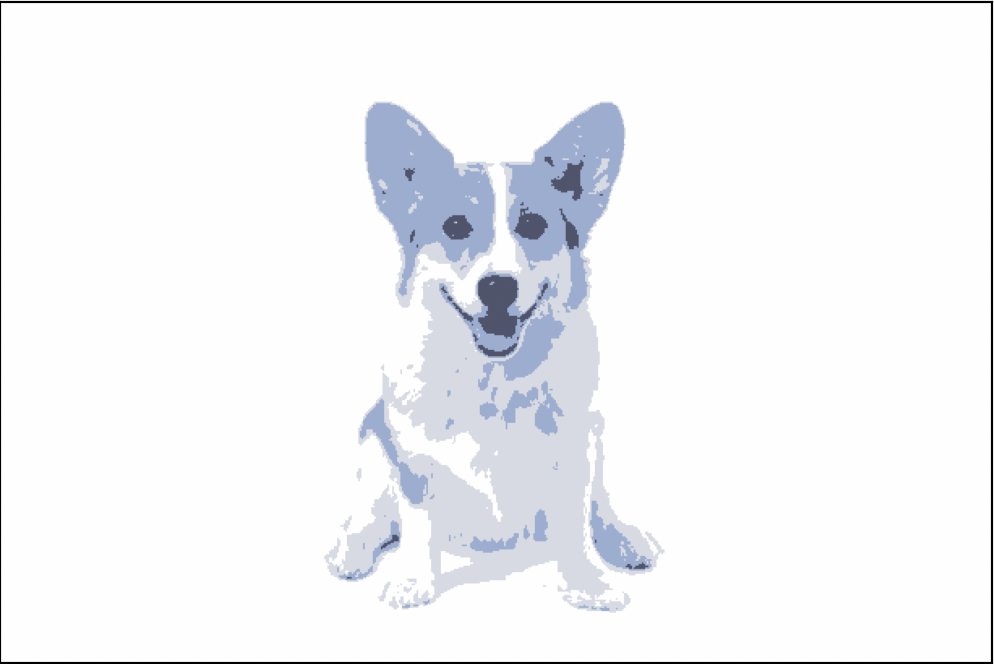
\includegraphics[scale=0.2]{corgi-white.png}
 \vspace{20px}
 \caption{The K-Means clustering algorithm (f=2 for Fuzzy C Means) applied to an image of a Corgi in a white back-ground.}
 \label{corgi:white}
\end{figure}

\begin{figure}[h]
 \centering
 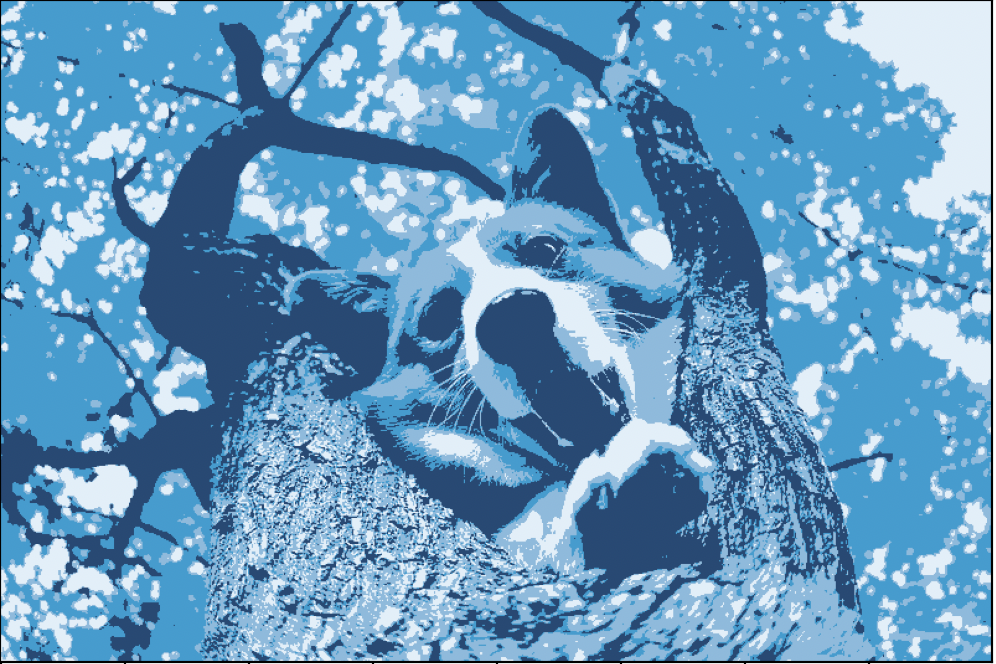
\includegraphics[scale=0.2]{corgi-tree.png}
 \vspace{20px}
 \caption{The same clustering algorithm applied to an image of a corgi on a tree. Note how pixels (i.e. colors) of the tree and Corgi get grouped together.}
 \label{corgi:tree}
\end{figure}


With this in mind, I plan to utilize a CNN that takes an input image of a given height, width, and three channels (\(Red, Green, Blue\)) and returns activations of features \( {f1, \cdots, fn} \) which will act as vectors of dimension \(n * f\), where f is the number of filters, for the Fuzzy C Means Algorithm. The convolutional neural network will have several convolutional layers which have 3 individual kernels/filters underneath (for each of the different color channels red, green, and blue). These kernels will be represented by a 3x3 matrix of set values as matrices for edges (called Sobel filters), which can detect edges and their corresponding spatial positions. The 2-D matrices will be mapped over the image by computing a given value for a given set of 9 (3x3) pixels for one channel (R, G, or B); computing this value will requiring the cross product or summing up all the multiplications of overlapping values of pixels and the filter together; this cross multiplication is known as the convolution operator. The values generated by convolution will represent the activation (i.e. if it detects the given feature, such as an edge). 

% However, an activation of 40 versus -10 can be seen as ambiguous and meaningless in terms of a single neuron (where we only care if it fires). 

% Upon the outputs of the kernels (called a feature map), they will be inserted into a ReLU activation function, which computes the activation (i.e. if the feature is recognized) based on if the value is positive (activates) or negative (doesn’t activate). After this convolutional layer and input through the ReLU function, the values are now simply activations or non activations. 

The second important layer of this convolutional neural network will be the max pooling layer, which in short allows for “translational invariance”, or the idea that if the image is rotated, sized differently, or viewed in different lighting \cite{Khandelwal2018}, that the object will still be recognized; this is necessary in the previously stated context of image manipulation. The max pooling layers will summarize the output of groups of pixels, by utilizing a matrix of size 3x3, taking the input from the previous layer and condensing it by selectively looking at a grid of pixels (the same size as the filter) and grabbing the maximum value of those pixels as its output. After moving horizontally across the image, to reduce computation, we can use a stride length of two, or basically to move two rows down vertically after moving across once. This reduces the size of the output and “pools” activations together. By reducing the size of input entering the next layer, it reduces the computational load, and by using max pooling (or grabbing the highest values only), it highlights the parts of the feature which most align with the given feature the kernel filter is trying to extract. As well as, by max pooling, this reduces overfitting (since we only look at general features by condensing rather than at outliers). The convolutional and pooling layer together form a "feature" (edge, color, position) detector which can derives whether a group of pixels has this feature, while reducing computational complexity, noise, and overfitting. 



With these layers in mind, the convolutional neural networks will have these convolutional and pooling layers interleaved, so that the convolutional layer uses convolution to find the filter and the pooling layer uses pooling to effectively “highlight” the activation it finds and reduce the size of the input image before it reaches the inner layers (where often you’ll be looking at smaller parts of an image). By convolution and pooling, I want to summarize the activation of a feature for a few distinct portions of the images.

The output of this final convolutional neural network will be a multi-dimensional matrix of pooled values representing varying amounts of activation \cite{Arc2018} and the number of filters applied to the image; to convert this into a datapoint, the matrix will be flatten into a single vector of a high number of dimensions. Normally, there would be a final layer, called the Fully Connected Layer (FC), which can be utilized to identify the object. However, given I want to simply cluster by similar objects and not identify them, omitting this final layer and placing the flatten vector into my clustering algorithm (FCM) is my preferred method. Fuzzy C-Means and K-Means are both computationally efficient at O(n) and O(knt) respectively \cite{Mittal2021}, and therefore utilizing either can save on computational costs, especially with the high number of pixels and features. 

Given the features from the CNN as an array of features \(f_{1} \cdots f_{n}\), the Fuzzy C-Means algorithm will look at these as a singular datapoint of dimension (or size) n, and cluster datapoints based on the Euclidean distance metric. 

% \begin{figure}[h]
% 	\centering
% 	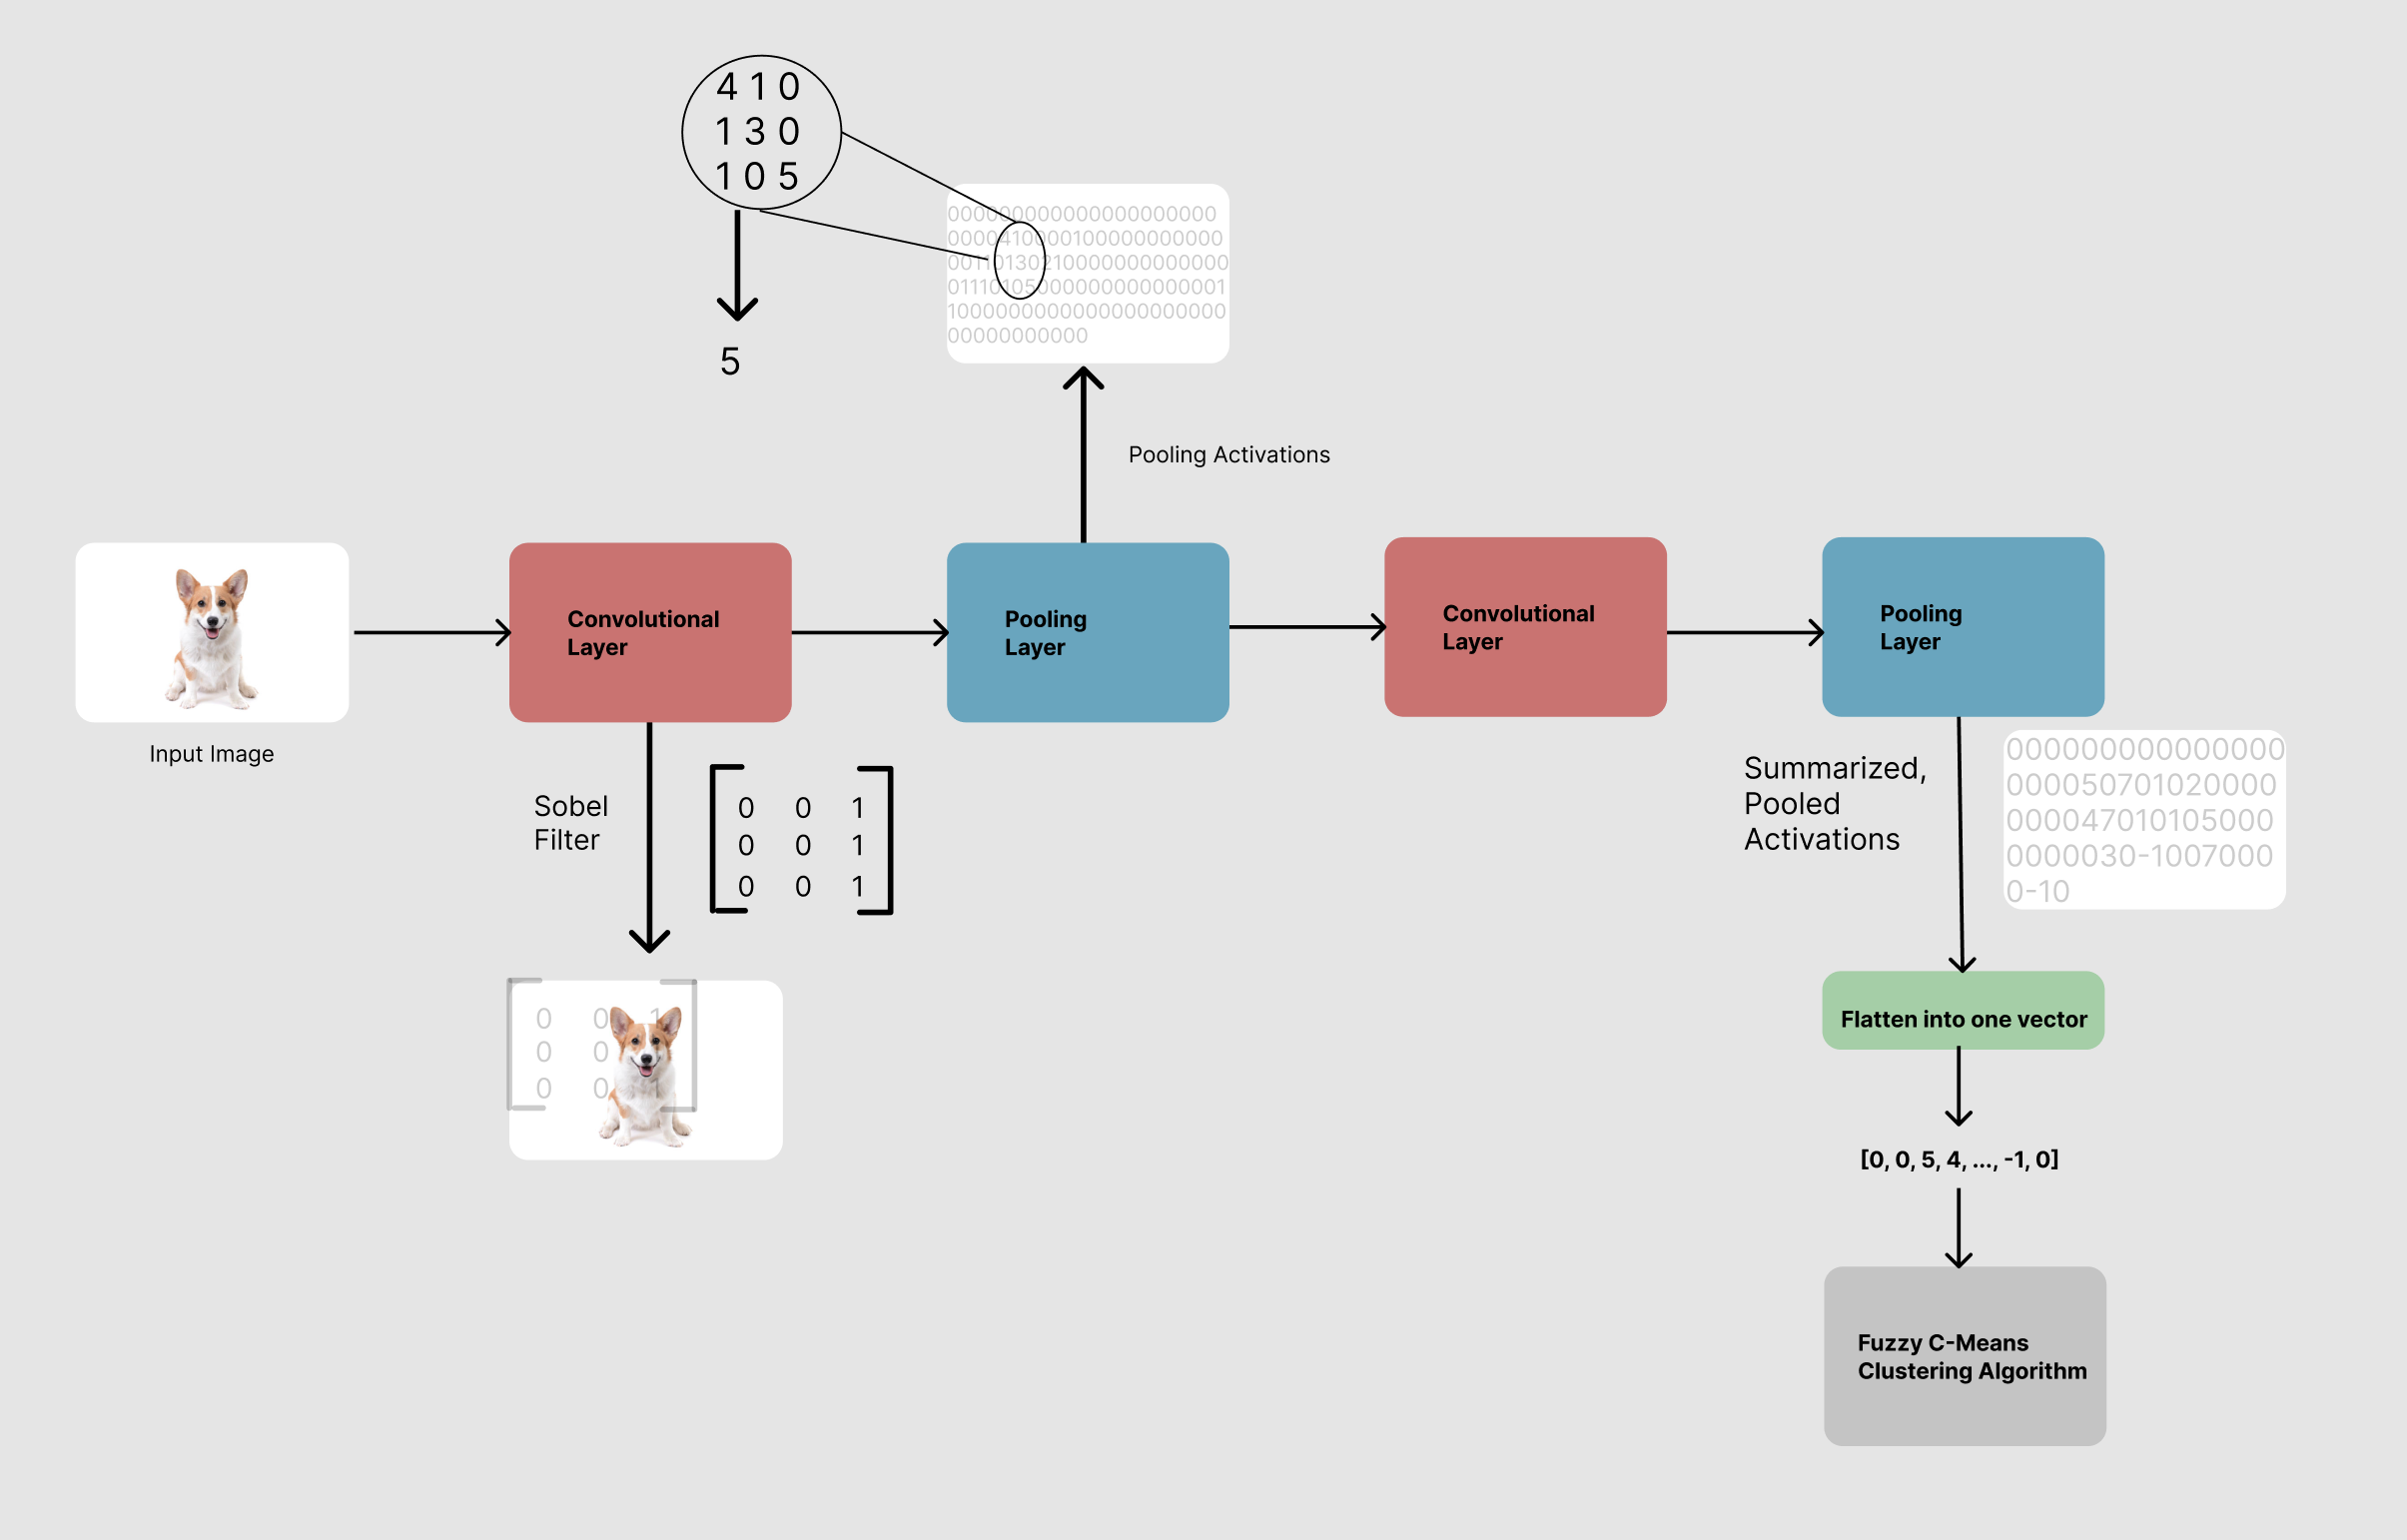
\includegraphics[scale=0.2]{CNN.png}
% 	\vspace{20px}
% 	\caption{A high-level diagram of the entire process.}
% 	\label{CNN}
%    \end{figure}

% The main idea behind the FCM algorithm is given all the data points and a fuzzifier (a number denoting how hard or soft the clustering is), to compute suitable centers of groups of videos/video frames based on a common feature or group of features that are similar between them. The output will be the positions of the centers of the centroids, and a corresponding table of the images and their corresponding clusters denoted by a number j. 

% \begin{algorithmic}
%   \begin{algorithm}
%     \State $f \gets $4
%   \end{algorithm}
	
	% \State $data_points \gets [f_1, f_2, …, f_n]
	% \State $centroids \gets [[0.1, 0.4, …, 0.05], …, k] 
	% \State $diff \gets $1
	% \While diff:
	% Calculate new centroid positions based on membership values of data_points
	% Recalculate the new membership values based on these new centroid positions compared to old ones
	% Calculate diff to be the difference between the original centroid position and new centroid position
	% If the diff is large enough, break
	
	% (Optional) Decide on a primary cluster for each datapoint depending on the largest membership it has
	
	% \Returns centroid positions, datapoint and corresponding clusters
% \end{algorithmic}

After these clusters have been computed, now the algorithm is set and ready to be tested. Placing a given image through the CNN gives us a relevant datapoint. Using this datapoint, we can determine initially what basket to check (by the Euclidean distance metric), as well as other viable options in order of membership value. Based on the data points distance to other data points, these corresponding images and video IDs will be returned first (since they are most similar in terms of visual characteristics). The progression of “relevance” will be determined by if the primary clusters are the same or not and then the corresponding distance to that datapoint. By computing this, we’ll get a list of videoIDs and their corresponding relevance depending on these factors. 

\section{Evaluation}

Not only does the evaluation of clustering algorithms allow us to test the cluster for the features/classes it groups upon, but it allows the developer (or myself) to identify and eliminate outliers, compare to human judgments, and understand the makeup of the data itself \cite{Lavrenko2014}. Within the context of this COMPS Project, evaluating the strengths and weaknesses of Fuzzy C-Means and K-Means clustering algorithms allowed me to introduce the idea of utilizing a convolution neural network.

To evaluate an image segmentation algorithm, it requires that we assess the strength of the clustering algorithm based on the meaningful classes that it generates. In other words, it should have clusters (even if they’re unlabeled), that resemble characteristics or blobs of image data that a human may draw out as meaningful. In our previous example, the Corgi in the tree, while clustered, was clustered into several different parts compared to just the Corgi in the white background. It’s clear that pixels do not serve as an identification for features, as colors can be shared by different parts or different objects within the image (in this case, the Corgi and the tree). There are mainly two parts I propose to evaluate a given clustering algorithm: the strength of these clusters (i.e. how well can it cluster pixels of an object together in comparison to a human) and how relevant are the videos to each other.

If we want to evaluate the strength of these clusters, there are several methods, but I propose utilizing combinations of comparisons between the prediction and ground truth such as Intersection-over-Union and a Confusion Matrix as these are not only widely used representations (making them easy for others to evaluate themselves based on the results) \cite{Mittal2021}, but they are not mathematically difficult to represent nor compute. Not to mention, it’s very easy to compare as we’re simply comparing pixel-to-pixel for clusters (as we’ll know all the pixels and their clusters given our methods) as opposed to instance segmentation which requires identifying the objects/classes.

A confusion matrix consists of representing the accuracy, precision, and recall based on storing the true values (true positive/negative) and negative values (false positive/negative) in a 2x2 matrix \cite{Jordan2018}. By utilizing formulas for accuracy, precision, and recall, we can define how accurate versus precise our clustering may be in relation to human judgment \cite{Jordan2018}. Rather than having to ask human judges to define the accuracy or even the cluster for us, we can determine how well it predicts the ground truth in comparison to previously human-segmented images. In turn, our evaluation can determine how strong the clustering algorithm can group similar features (and therefore similar videos) together without having to ask for human judgment.

While the clustering algorithm may be solid for determining images of related visual similarity, the last question to ask is whether these clustering algorithms lead to related videos (of most importantly related content). As computers cannot evaluate the similarity between videos based on content, my plan is to ask others to test the program with test images of their own (and my own) and determine whether the related videos are helpful or not. As the primary user may be a student or researcher, I may ask for related lecture notes, diagrams, and drawings with the intent of assessing the relevance of the videos my program generates. While this may be qualitative, a quantitative judgment such as those in the previous paragraph, may not be able to measure helpfulness due to a disparity between the video image similarity and the video content similarity.

\section {Ethical Considerations}

% - less extreme on proposal of ethics
% - that are most relevant 
% - dw about image manipulation
% - (dias)selection bias
% - warning based on keywords of videos
% 	- human segmentations?

% The project is considered both in its complete technological and societal context. 
% Issues of bias and diversity are explored in detail, and potential contributions to global and local inequity examined. 
% Relevant literature is cited.

In consideration of the ethical aspects of this project, there are aspects of the data and algorithms which have bias including the Youtube 8M Dataset, the clustering algorithm, and convolutional neural network.

In the process of creating this project, there are ethical concerns of this project such as the bias within the data used for the CNN and clustering, as well as, a lack of explainability and transparency entirely behind my algorithm.

To begin with, the YouTube 8M Dataset primarily contains selection bias and sample bias due to the limited amount of data and diversity surrounding video platforms and YouTube 8M’s dataset. Selection bias, to be general, is the difference in characteristics between those selected for a study (training data) and those not (test / real world data) \cite{Yu2020}; YouTube’s 8M Dataset, which contains 6.1 million videos from 2017 and 2018 \cite{googleYT8M}, has much less data compared to the estimated 800 million on Youtube. While the dataset contains the data across the same amount of general categories (15), the distribution of data across these categories and subcategories is weaker, primarily having videos in the games or vehicle category \cite{googleYT8M}. This combination of lack of data and diversity within the data contributes to poor generalization, or poor performance on the test set (real world) in comparison to the training set, due to the model overfitting to the training data and struggling to account for new characteristics from new input images \cite{Yu2020}. The main reason behind poor generalization in selection bias comes from unwanted correlations between features or characteristics in images; clustering on images with these correlated features lead to “spurious (fake) relationships” \cite{Yu2020}. Furthermore, due to the selection of data by YouTube, the YouTube dataset has sample bias and a favoring toward Western ideals. To reiterate, the videos from the dataset are primarily distributed in games, vehicles, and concerts with around 780,000 videos, whereas only 3000 videos are available about Indian cuisine and TV. The major advertising audience from YouTube is aged 25-34, male, and from India \cite{HootSuite2022}; despite this, there is a disparity in content and data surrounding India.

As a final point, due to the lack of explainability behind the machine learning algorithm’s decisions, finding and fixing the sources of unethicality (bias) can become an ethical issue. While many machine learning algorithms, Fuzzy C-Means included, are mathematically explainable in how they converge or determine clusters, these explanations don’t describe why they decided on a specific set of clusters. As a consequence of this implementation, fixing a known source of bias and error, through fixes in the implementation, is difficult; telling the computer where the centers should be removes the machine learning aspect of this project.




% Selection bias, to be general, is the difference in characteristics between those selected for a study (training data) and those not (test / real world data) \cite{Yu2020}; it primarily occurs due to an underrepresentation of the population from the sample. YouTube’s 8M Dataset, which contains 6.1 million videos from 2017 and 2018 \cite{googleYT8M}, has much less data compared to the estimated 800 million on Youtube. While the dataset contains the data across the same amount of general categories (15), the distribution of data across these categories and subcategories is weaker, primarily having videos in the games or vehicle category \cite{googleYT8M}. While YouTube has the same number of categories, they are meant to encompass many of the videos together; the subcategories (and more niche categories) of YouTube beneath these general categories are not shown or displayed (more inferred and created by subcommunities). This combination of lack of data and diversity within the data contributes to poor generalization, or poor performance on the test set (real world) in comparison to the training set, due to the model overfitting to the training data and struggling to account for new characteristics from new input images \cite{Yu2020}. The main reason behind poor generalization in selection bias comes from unwanted correlations between features or characteristics in images; clustering on images with these correlated features lead to “spurious (fake) relationships” \cite{Yu2020}. A great example is working with an image dataset containing images of mainly dogs laying in grass. Upon the introduction of an image of a cat laying in grass, due to the high correlation between dogs and grass (implicitly in the data), the cat gets placed in the wrong cluster with the dogs \cite{Wang2020}. In a similar fashion, any unintentional and intentional biases of the YouTube 8M dataset will be exacerbated, by the model conforming to what it believes is the population (training data) and forming relationships (such as between dogs and grass) about this data which don’t exist on all of YouTube. The subtypes of selection bias, historical and sample bias, can further describe the specific limitations and contribution effects of bias in our data and why our data cannot be ethical when used for machine learning.

% Finally, due to the selection of data by YouTube, the YouTube dataset has sample bias and a favoring toward Western ideals. To reiterate, the videos from the dataset are primarily distributed in games, vehicles, and concerts with around 780,000 videos, whereas only 3000 videos are available about Indian cuisine and TV. The major advertising audience from YouTube is aged 25-34, male, and from India \cite{HootSuite2022}; despite this, there is a disparity in content and data surrounding India. Part of the reason behind the creation of the dataset was addressing the need for “large-scale, labeled datasets” and “[accelerating] research on large scale video understanding” \cite{Warrick2020}. As gaming and car content thrives on YouTube, this data may’ve been curated to not only appeal to Western developers, but to bring research on the largest sources of videos. Additionally, as the data is human-labeled \cite{googleYT8M}, only those from Google who had the technology and expertise to label the data did so. In the process, this disfavors content and people (who would label) from other backgrounds and lessens the diversity of the data. This selection of data affects the clustering algorithm in a similar way to sample bias, or bias due to nonrandom data. Like selection bias, sample bias will cause correlation between features; as non-popular videos (due to language or cultural barriers) are less likely picked (and have small groups), it’s less likely the clustering algorithm will create a separate cluster for them. In the process, the algorithm is less likely to group objects and people from lesser-known videos/backgrounds together, instead placing them in a larger cluster (from some other identifying feature) with less related videos. Additionally, the algorithm may choose to focus on a well-known feature of a lesser-known video as opposed to a lesser-known, identifying feature of the video or thumbnail. As a result, finding related videos for an object or person not recognized in the United States becomes more difficult (and may even require parsing through the relevant videos by the user which defeats the purpose). Evidently, the unintentional biases present within my data contribute to the algorithm making incorrect relationships in the data and unethical decisions (clusters) based on its interpretation of the population.

% As a final point, due to the lack of explainability behind the machine learning algorithm’s decisions, finding and fixing the sources of unethicality (bias) become too tedious and difficult to handle. While many machine learning algorithms, Fuzzy C-Means included, are mathematically explainable in how they converge or determine clusters, these explanations don’t describe why they decided on a specific set of clusters. For the Fuzzy C-Means algorithm, as the initial centers of centroids are picked at random and the placement of these initial centers affects the end result, there’s no way to backtrack mathematically. The algorithm can perform very well or very poorly, and the best method of overcoming this simply involves recomputing the clusters until the error (or distance between the cluster’s centroid and its corresponding distance) is minimized \cite{GeeksForGeeks2019}. As a consequence of this implementation, fixing a known source of bias and error, through fixes in the implementation, is difficult; telling the computer where the centers should be removes the machine learning aspect of this project. As well as, if and when my algorithm acts unfairly, I cannot determine the source of its decision whether it’s due to the data or implementation of my algorithm. While I can reiterate and determine a relatively good set of clusters (using methods like the Elbow method to evaluate them \cite{PrasadClustering}), this doesn’t ensure optimal or unbiased results. This translates to deployment where the algorithm may perform horribly and under new data, return unexpected results without any sort of way to determine where it went wrong. The main solution to this problem is either removing the root cause (if it’s findable), or removing the project from deployment immediately (like with Microsoft’s Zo). As finding the root cause of an unethical decision/result is difficult, neither of these decisions are sufficient for completing and deploying my project. Either I have to micromanage the algorithm (which defeats the purpose of it being machine learning), or I have to start from scratch with the data and algorithm (which already has presented problems). In total, unintentional and intentional data biases present themselves as unavoidable and difficult ethical issues to fix; finding and fixing all of these is not doable given the scope of my project.



\section {Proposed Timeline}

The proposed timeline will be split into two parts: the summer (late May to late August) and the fall (early September to early December); each of these parts will be discussed in brief (1 to 2 sentence) two-week (half-month) segment plans.

During the summer, the second half of May will be a reflection while the ideas of the methods, algorithms, and evaluation methods are still fresh in my brain. I'll look deep into my design decisions and identify where questions are weakly answered in terms of design, understanding, and implementation and focus harder on these; the areas which are harder to explain and implement are answers in need of focus first. During the first half of June, a simple, but crucial area of focus will be the data I'll be utilizing, and determining how to gather, process, and input the raw videos and ideally video frames. During the second half of June, my next crucial area of focus will be the full understanding of the convolutional neural network and the appropriate number of filters, layers, input images, and outputs of the CNN. I'll read upon how to implement and evaluate them, as well as the ethics or weaknesses of the CNN. As I expect this will be a large task, during the first half of July, I'll continue my search of knowledge with CNNs and look into other Sobel filters, neural network layers, and computation layers that can help with processing and segmentation for different, useful features. During the second half of July, given the inputs and outputs of the CNN are more solidified, I'll bring attention to the clustering algorithm and determine the viability to cluster over such high dimensions of datapoints and other better approaches of clustering that don't utilize a distance metric (if they're better and work better with CNNs). During the first half of August, I'll focus on the evaluation and ethical considerations of the methods, design, and implementation I've solidified, and jot ideas of how to evaluate (both in terms of output and ethics) based on other papers and sources of information. During the last half of August (before school starts), this will be a vacation away from this project. After working on the ideas of this project as well as completing an internship, I think stepping back and preparing for the full implementation and rush will be a smarter approach; this may involve looking at my project over from a bird's eye view. 

% By the end of the summer, I should have a deeper understanding of how the inputs and outputs will be processed and computed accordingly, in design, evaluation, ethics, and implementation (most to least important). Or, I should have a new idea if the COMPS idea I proposed before isn't doable in the given time frame. As a whole, the goal of the fall is to put my ideas into fruition, which in the context of software bugs and unexpected "walls" will be difficult; having the design, evaluation, and ethics set into place will make the implementation (which is more important during the school semester) easier in the long run.

Beginning in the fall, in the first half of September, the main task at hand is constructing the convolutional neural network and determining how, in code, the image will be read, segmented, and converted into an array of activations of features (outputs). As this is the most important and difficult part of project (I expect), this is the initial barrier to overcome and I suspect this may take longer. In the second half of September, I'll continue this implementation process further, while beginning to focus on the implementation of clustering and determining the bridge converting the "datapoints" from the CNN into many grouped, fuzzy clusters. In the first half of October, I'll look into implementing or designing how an input image will be inserted and how the relevant videos will be calculated and generated. Further, I'll look into how to evaluate the several different components created in September and how to evaluate the outputs based on relevance as well as ethics. In the second half of October, I'll continue to test and solidify my implementations in September, by giving videos from the YouTube8M Dataset into the CNN and creating clusters with my implemented clustering algorithm. If the clusters are being created successfully, I'll begin to input and test my videos further and determine if the outputs (related videos) make sense. In the first half of November, with several parts implemented and some testing complete, I'll begin drafting and determining the design of my poster, mainly how to describe the design, implementation, and evaluation in a brief, but descriptive manner. In the second half of November, I'll begin to finalize my project and test/debug the corresponding components accordingly. As well as, I'll look into ways to present the project besides just talking about it, whether through showing it with my computer or making a very simple web app (such as with little CSS, and simply a way to input images and show the outputs). In the first half of December, I'll finalize all my ideas, reread and rewrite parts of my paper to reflect the complete design, implementation, ethics, discussion, and other sections of the paper. I'll look into my code and clean up the README, folders/files, and code to make it navigable and understandable (design and implementation-wise).  






\printbibliography


\end{document}
